% CONCLUSIONS
\chapter*{Synthèse et perspectives}
\markboth{Synthèse et perspectives}{}
\addcontentsline{toc}{chapter}{Conclusions et perspectives}
\newpage

%L'étude des flux de carbone dans les écosystèmes tourbeux est complexe car assujetti à des facteurs de contrôle dont la prépondérance varie fortement selon l'échelle considérée et les conditions environnementales.
%Les effets d'un facteur contrôlant sur un flux de gaz vont généralement dans le même sens dans la littérature : 
%une hausse de la température à tendance à augmenter les flux.
%Une augmentation du niveau de la nappe à tendance à favoriser la production de \chh par rapport à celle du \coo.
%La végétation semble faciliter les échanges de gaz et libère des substrats facilement mobilisables.
%Outre le fait que ces facteurs co-varient et qu'il donc difficile de distinguer leurs effets, ces effets sur les différents flux en terme de bilan de carbone est beaucoup moins nette, d'où la nécessité d'estimer des bilans de carbone sur ces écosystèmes.


%Le devenir des tourbières, de leur fonction de puits et de leur stock de carbone accumulé pendant les derniers millénaires, reste incertain.
%Ces travaux se sont focalisés sur l'étude d'une tourbière de Sologne (la tourbière de La Guette), envahie par une végétation vasculaire.
%L'intérêt de son étude réside dans cette problématique de perturbation anthropique probablement liée à cet envahissement.
%Mais également sa position à la limite sud de l'extension des tourbières à sphaignes de l'hémisphère Nord, qui la place dans des conditions limites, moins favorable a priori au développement de ces écosystèmes.

À l'échelle globale les tourbières s'étendent sur des surfaces limitées, mais elles jouent un rôle important de part leur fonctionnement comme puits de carbone.
Ces écosystèmes subissent des perturbations anthropiques et climatiques qui rendent incertain le devenir du stock de carbone qu'elles ont accumulées pendant les derniers millénaires.
Les facteurs qui contrôlent les flux de carbones qu'elles échangent avec l'atmosphère sont globalement connus (température, végétation, hydrologie) mais leurs effets nécessitent encore d'être compris plus en détails

Nos travaux ont été orientés selon deux approches : l'observation, qui permet de comprendre le fonctionnement puits/source d'un écosystème (La tourbière de La Guette), et l'expérimentation qui permet l'étude plus spécifique d'un facteur de contrôle, ici l'hydrologie.

\section*{Synthèse générale}


\subsection*{Le bilan de carbone}

L'estimation du bilan de carbone de la tourbière de La Guette montre que l'écosystème fonctionne comme une source de carbone.
Sur les deux années de suivi elle a ainsi perdue \SI{220(33)}{\gcma} malgré un niveau de nappe d'eau proche de la surface du sol.
Ce bilan est contrôlé en grande partie par les émissions de \coo qui sont deux ordres de grandeur au dessus de celles du \chh et du COD.
Si on schématise ce bilan on considérant 100 atomes de carbone qui entrent dans la tourbière (PPB) on a :

\begin{equation}
100C_{PPB} \rightarrow 118C_{RE} + 2C_{\chh} + 1C_{COD} -21\Delta C
\end{equation}

Soit 118 atomes de carbone émis sous forme de \coo respiré, 2 sous forme de \chh et 1 sous forme de COD et un déficit de 21 atomes.
Pour expliquer ce bilan négatif trois points sont à considérer.

Le premier concerne les températures moyennes annuelles du site qui sont élevées par rapport à d'autres tourbières.
Ces températures entraînent des flux importants qui se traduisent avec une importance forte dans le bilan en cas de déséquilibre.
En effet les estimations des flux de \coo entre la tourbière de La Guette et l'atmosphère, sont dans la tranche haute des émissions relevées dans la littérature que ce soit pour la RE (\SI{1261(164)}{\gcma}) ou la PPB (\SI{1070(203)}{\gcma}).
La tourbière subit également un climat moins dur avec des hivers moins longs et froids que celles situées à plus hautes latitudes, ce qui permet aux flux de rester plus élevés pendant une période de l'année plus longue.
Il semble donc cohérent que les flux de \coo estimés soient plus fort que ceux mesurés dans des tourbières boréales.

Le second point est lié au premier : la tourbière de La Guette est située en plaine. 
Elle ne profite pas des été plus frais et humides et des hivers plus froids d'un climat montagnard et ses flux de RE restent important même la nuit et l'hiver.
On peut ainsi comparer le premier jour des mesures haute fréquence entre les sites de Frasne et de La Guette (cf chapitre~\ref{ch:ch5}, Figure~\ref{fig:er_tair_tpeat}).
Malgré des températures en journée plus élevées sur le site de Frasne, la RE mesurée est plus faible que ce soit la nuit ou le jour.
%Les flux mesurés à Frasne ont un maximum moins élevé le jour et un minimum plus bas la nuit, alors que les température de l'air maximum de la journée sont plus forte à Frasne.
%(Limites de la comparaison : mesure à un temps différent)

Le troisième point est la présence d'une végétation vasculaire herbacée, ubiquiste, adaptée aux milieux inondés pouvant maintenir une activité photosynthétique et de respiration autotrophe même dans des conditions de niveau de nappe d'eau élevé.
Les estimations des flux de \coo se rapprochent de celles estimées dans les tourbières utilisées comme prairies permanentes, sans toutefois les atteindre.
Cette comparaison a du sens car la tourbière de La Guette, est fortement envahie par une herbacée (\textit{Molinia caerulea}) largement dominante.
Ceci semble également cohérent car ces écosystèmes ont généralement une végétation herbacée majoritaire, mais un niveau de nappe d'eau plus bas favorisant des flux plus fort, notamment pour la respiration.

Le bilan est donc contrôlé en grande partie par le \coo mais les flux de \chh estimés sont également importants (\SI{17(5)}{\gcma}) et plutôt dans la tranche supérieure des valeurs relevées dans la littérature, ce qui est cohérent avec le niveau de nappe d'eau proche de la surface du sol relevé sur le site pendant les deux années de mesure.
Enfin les flux de COD sont plutôt faibles par rapport aux données relevées dans la littérature.
Ce flux est contraint principalement, sur les deux années de mesures, par la quantité d'eau qui quitte l'écosystème supérieure en 2014 par rapport à 2013.

Les bilans estimés pour les années 2013 et 2014 différents : la tourbière de La Guette est une source plus importante en 2013 (\SI{-301(47)}{\gcma}) qu'en 2014 (\SI{-138(20)}{\gcma}).
Les valeurs de la RE sont proches pendant les deux années et cette différences semble davantage être causée par une hausse de la PPB de \num{957(182)} à \SI{1184(225)}{\gcma} entre 2013 et 2014.
Ce constat est à mettre en parallèle avec l'histoire de la tourbière qui sort de plusieurs années de bilan hydrique négatif et d'assèchement important.
Le niveau de la nappe d'eau était élevé dès de début des mesures, cependant il est possible que les capacités de développement et de photosynthèse de la végétation soient encore amoindrie en 2013.
\textbf{(Corroboré par mesure par groupe)}




%\subsection*{Intensité des flux sur la tourbière de La Guette}

%%\subsubsection{Intensité des flux sur la tourbière de La Guette}
%Les estimations des flux de \coo entre la tourbière de La Guette et l'atmosphère, sont dans la tranche haute des émissions relevées dans la littérature que ce soit pour la RE (\SI{1261(164)}{\gcma}) ou la PPB (\SI{1070(203)}{\gcma}).
%Il semble cohérent que les flux de \coo soient plus fort que ceux mesurés dans des tourbières boréales.
%De par sa position géographique, le site à une température moyenne annuelle élevée par rapport à la majorité des écosystèmes tourbeux (Figure~\ref{fig:bib_vs_necb}.).
%La tourbière subit également un climat moins dur avec des hivers moins longs et froids que celles situées à plus hautes latitudes, ce qui permet aux flux de rester plus élevés pendant une période de l'année plus longue.
%Les estimations des flux de \coo se rapprochent de celles estimées dans les tourbières utilisées comme prairies permanentes, sans toutefois les atteindre.
%Cette comparaison a du sens car la tourbière de La Guette, est fortement envahie par une herbacée (\textit{Molinia caerulea}) largement dominante.
%Ceci semble également cohérent car ces écosystèmes ont généralement une végétation herbacée majoritaire, mais un niveau de nappe d'eau plus bas favorisant des flux plus fort, notamment pour la respiration.


%Les flux de \chh estimés sont également importants (\SI{17(5)}{\gcma}) et plutôt dans la tranche supérieure des valeurs relevées dans la littérature, ce qui est cohérent avec le niveau de nappe d'eau proche de la surface du sol relevé sur le site pendant les deux années de mesure.
%%Ces observations sont cohérentes avec le niveau de nappe d'eau haut relevé sur le site pendant les deux années de mesure qui a contribuer à minimiser l'oxydation du \chh pendant son transport vers l'atmosphère.
%
%Enfin les flux de COD sont contraint principalement, sur les deux années de mesures, par la quantité d'eau qui quitte l'écosystème supérieure en 2014 par rapport à 2013.

\subsection*{Variabilité spatiale des flux}

Ces travaux ont également montrés la forte variabilité spatiale des flux de \coo sur la tourbière de La Guette.
%À notre connaissance il n'existe pas d'estimation de la variabilité spatiale des flux de \coo à l'échelle d'un site 
Sur les \SI{13}{\hectare} de la tourbière active, la variabilité spatiale des flux de \coo s'étend sur une gamme aussi importante que celle visible à l'échelle de l'hémisphère nord entre différents sites (Figure~\ref{fig:vs_bib}--A et B).
Les estimations de bilan dépassent même la gamme les valeurs relevées dans la littérature (Figure~\ref{fig:vs_bib}--C).
Ces résultats soulignent l'importance de la variabilité spatiale et de la nécessité de la considérer lors du développement de protocoles de suivi des flux de GES.
Concernant le \chh, le nombre limité de points de mesure ne permet pas de faire le même type de comparaison.

Paradoxalement les zones de la tourbières fonctionnant en puits de carbone sont celles ou les herbacées sont dominantes.
L'explication de cette observation reste incertaine.
Il est possible que le potentiel de photosynthèse de l'écosystème, et plus particulièrement celui des sphaignes ne soit pas à son maximum après les années sèches qui ont précédé les mesures.
%Dans cette hypothèse, la réhumectation de la tourbière aura également pu piéger une partie du \coo produit les années précédentes
%Le niveau de la nappe d'eau, proche de la surface du sol, à peut être mini

\subsubsection{Effet de l'hydrologie sur les flux de GES}

Même si les faibles variations du niveau de la nappe d'eau mesurée sur la tourbière de La Guette pendant les deux années de mesure n'ont pas permises de les relier directement aux émissions de GES, l'hydrologie joue un rôle important.
%Ainsi le niveau de nappe élevé en 2013 et 2014 explique probablement

D'abord l'importance de flux de \chh, dont l'estimation est plutôt dans la tranche supérieure des valeurs relevées dans la littérature, est probablement liée au niveau de la nappe d'eau.
Ce dernier en étant proche de la surface du sol empêche l'oxydation du \chh.
Le fait d'avoir des flux plus faible en 2013, année ou le niveau de nappe a légèrement baissé en été, qu'en 2014 va dans le même sens.
Suite aux expérimentations sur mésocosmes, il semble d'ailleurs qu'à niveau de nappe d'eau élevé, la proportion aérobie/anaérobie de la colonne de sol ne soit plus le processus prépondérant de contrôle des émissions de \chh.

%? au dessus de -10 limitation car limitation de la photosynthèse ? (semble pas particulièrement minimiser dans chap4)

Ensuite malgré un niveau moyen de la nappe d'eau plus élevé en 2014 qu'en 2013, l'estimation de la quantité d'eau sortant de la tourbière est également supérieure en 2014.
Cette inconsistance apparente s'explique probablement par l'histoire de la tourbière pendant les années précédents les mesures.
En 2011 et 2012 la tourbière a subit un étiage important et s'est vidée d'une part importante de son eau, suffisante pour pouvoir s'y déplacer sans bottes (Sébastien Gogo, communication personnelle), ce qui n'est jamais arrivé en 2013 et 2014.
En 2013 une partie importante de l'eau arrivant dans la tourbière a donc servie à la renflouer, cette part l'est beaucoup moins en 2014 la tourbière étant déjà en grande partie « en eau ».
Ces variations dans la décharge en eau de la tourbières sont la source des différences d'estimation du COD entre 2013 et 2014.
%Cette histoire semble expliquer les estimations des flux de COD, supérieur en 2014.

Enfin, même si aucune tendance directe n'est visible avec les flux de \coo, le niveau de la nappe d'eau particulièrement élevé pendant les deux années de mesure a probablement eu un rôle.
Notamment il a pu limiter un peu les flux de RE en minimisant la proportion aérobie de la colonne de tourbe.
Malgré tout les flux observés sont important, cela peut s'expliquer car à la fois \textit{Molinia caerulea} et \textit{Eriophorum Augustifolium} possèdent un aérenchyme, cette adaptation aux milieux inondés, qui leur permet de maintenir des échanges gazeux de leurs racines à l'atmosphère.
Son effet est davantage visible sur les expérimentations sur mésocosmes, ou un niveau de la nappe d'eau plus bas entraîne une augmentation des émissions de la RE.
%Les flux de \chh ne semblent quant à eux pas être contraint par le niveau de la nappe pendant les deux années de mesures.
%Leur relation avec la végétation laisse encore une fois penser un effet possible de l'aérenchyme.

%\subsubsection{Contrôle du COD}


\subsection*{Les modèles}

\subsubsection{Intérêt de l'évaluation}
%Cette force des flux de \coo est probablement liée à sa situation géographique locale et globale : une tourbière de plaine située à basse latitude et à ses problématiques de drainage et d'envahissement par une végétation vasculaire.
%Ainsi la saisonnalité plus faible qu'en montagne permet aux flux de rester fort pendant une période de l'année plus importante.
%Ces flux importants entraînent des variations forte en terme de bilan selon les méthodologies employées, il est cependant probable que la tourbière de La Guette fonctionne actuellement comme une source de carbone.

%L'estimation du bilan à l'échelle saisonnière ne permet pas de reproduire les variations journalières, l'estimation du modèle pendant les 3 jours de mesures haute fréquence réalisés en 2013 est largement supérieure aux valeurs mesurées (Figure~\ref{fig:RE1_vs_JN})

Que ce soit pour la PPB ou la RE, la prise en compte de la végétation améliore la calibration des modèles.
Pour la PPB l'intégration de la végétation n'améliore pas l'évaluation du modèle.
Ceci indique que, si d'autres suivis du même type sont effectués sur le site, l'estimation des flux de PPB en intégrant la végétation est à étudier à nouveau et ne va pas de soi.
De plus l'intégration de la végétation dans l'estimation des flux de PPB à un effet important qui change le bilan final de l'écosystème.
À l'inverse pour la RE l'intégration de la végétation, qui améliore également l'évaluation, ne change de façon importante l'estimation du flux de carbone.
Son utilisation pour estimer les flux de RE d'autres suivis du même type sur la tourbière de La Guette semble pertinent.
Enfin l'estimation du \chh, dont l'évaluation montre une erreur importante, doit être limité à l'estimation d'un ordre de grandeur des flux émis lors de ce suivi en particulier.
Ces résultats montrent l'intérêt fort de l'évaluation des modèles utilisés pour pouvoir préciser leur limites d'utilisation mais également les limites dans les interprétations qu'ils permettent.

La prise en compte de la végétation reste une difficulté importante, l'observation répétée nécessitant des mesures non destructives, souvent imprécises ou très coûteuses en temps.


\subsubsection*{Modélisation saisonnière et mesures horaires}

Les estimations des flux de la tourbière de La Guette par les modèles du chapitre~\ref{ch:ch3} ont été calculées à l'heure.
Elles ont donc pu être comparées aux données acquises sur le même site lors d'autres expérimentations, notamment grâce à l'utilisation de méthodes de mesures identiques sur l'ensemble de ces travaux.
Ainsi si l'on compare la RE estimée à l'aide des modèles RE-1 et RE-3 (chapitre~\ref{ch:ch3}) aux données acquises à haute fréquence (chapitre~\ref{ch:ch5}) on observe un écart important entre les valeurs mesurées et celles estimées par les modèles (Figure~\ref{fig:RE1_vs_JN}).
Pour expliquer cet écart on peut considérer les deux points suivants : 

Premier point, on compare des modèles qui prennent en compte la variabilité spatiale du site (une partie au moins, à travers les vingts points qui on servi à les calibrer) à des mesures réalisées sur quatre embases dans une zone restreinte de la tourbière (20 x \SI{20}{\metre}).
Ces quatre points ayant une représentativité spatiale limitée et ont été choisi pour leur similarités.
Cet écart peut donc être en partie le reflet de la variabilité spatiale des flux dans la tourbière.
Cet argument est soutenu par les mesures de RE réalisées le 24 et le 25 juillet 2013, soit 5 jours avant les mesures haute fréquence et dont la gamme de valeur est comprise entre \num{4.8} et \SI{18.9}{\uml} et sont représentés par le fond gris sur la figure~\ref{fig:RE1_vs_JN}.
Les estimations des modèles RE-1 et RE-3 restent d'ailleurs majoritairement dans cette gamme de valeurs.
Par ailleurs, la placette p04 (Figure~\ref{fig:carteVS}) la plus proche des mesures haute fréquences, est dans la gamme basse des flux que ce soit pour la campagne du 24-25 juillet : troisième flux le plus faible mesuré (\SI{6.1}{\uml}) ou en moyenne sur l'ensemble de mesure ou elle vaut \SI{2.81(160)}{\uml} par rapport à la moyenne de l'ensemble des placettes valant \SI{3.77(289)}{\uml}.

Second point, le modèle est calibré à partir de moyennes des flux par campagne de mesure (Figure~\ref{fig:flux_evolution_avg}--A et B).
Ces moyennes sont comprises entre \num{0.69(027)} et \SI{9.43(348)}{\uml}, par conséquent les estimations des modèles, dont RE-1, en dehors de cette gamme sont du domaine de l'extrapolation et donc à considérer avec précaution.

\begin{figure}
\centering
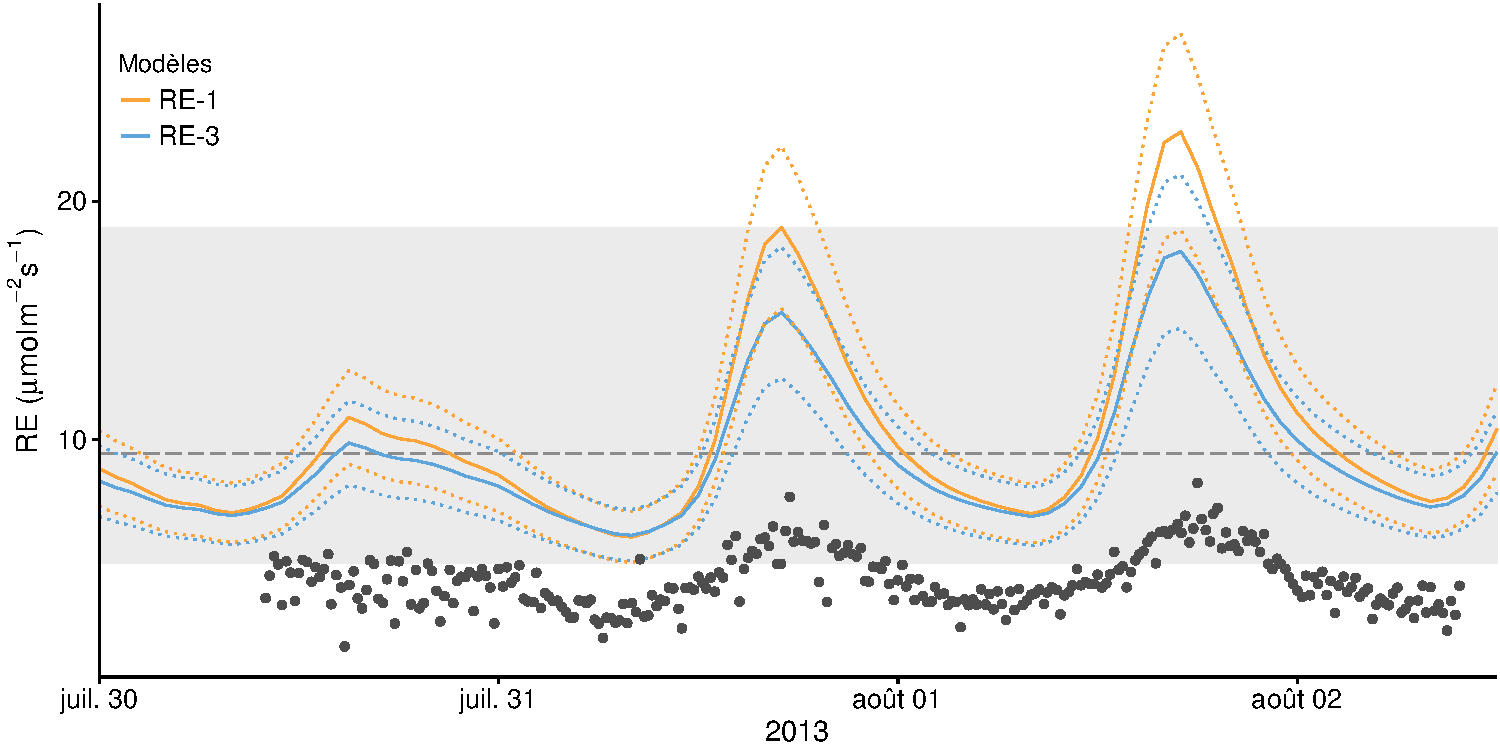
\includegraphics[width=1.15\textwidth, center]{conclusions/RE1_vs_JN}
\caption{Comparaison entre les valeurs estimées par les modèle RE-1 (ligne orange), RE-3 (ligne bleue) et les mesures faites à haute fréquence sur le site du 30 juillet au 2 août 2013 (points noirs). Les lignes de pointillés représentent l'erreur (NRMSE) associée aux modèles. La zone grisée correspond à la gamme de valeur de la RE mesurée sur l'ensemble des 20 placettes pendant la campagne du 24-25 juillet 2013. La ligne de tiret correspond à la moyenne de la RE pour cette campagne.}
\label{fig:RE1_vs_JN}
\end{figure}

Ces deux points considérés, il semble que les estimations des modèles RE-1 et RE-3, malgré les écarts que l'on peut observées, restent cohérentes avec les mesures effectuées aux différentes échelles.
Le modèle RE-3 restant davantage encore que le modèle RE-1 dans la gamme de valeur attribuable en grande partie, à la variabilité spatiale.
Cette comparaison montre également l'importance de la variabilité spatiale des flux dans les tourbières et la difficulté qu'il peut y avoir à la prendre en compte de façon satisfaisante.



\section*{Perspectives}

Sur les données acquises pendant ce travail, un certain nombre de points mériteraient d'être approfondi.
Ainsi il serait intéressant d'explorer le détail des relations flux de GES/facteurs contrôlant pour chaque placette.
Ceci permettrait d'estimer si la variabilité spatiale observée est plutôt liée à une différence de sensibilité avec des facteurs contrôlant identiques, ou si elle est plutôt liée à une différence dans la prépondérance des facteurs contrôlant.
Certaines placettes plus sensibles à la baisse du niveau de la nappe d'eau en 2013 gagneraient peut être à l'inclusion du niveau de nappe dans leurs estimations.

Continuer de suivre les flux de GES et d'estimer le bilan de carbone de l'écosystème à plus long terme semble également indispensable afin de comprendre comment fonctionne le système vis-à-vis de processus dont l'amplitude temporelle est plus importante.
Par exemple la variation inter-annuelle des températures, des précipitations, du niveau de la nappe ou les variations des communautés végétales.
Ce suivi sera probablement fait dans le cadre du SNO Tourbière et de l'installation prochaine d'une tour Eddy Covariance permettant de mesurer les flux à plus haute fréquence et de façon continue (aux contraintes de la méthode près).
Idéalement une année commune de suivi spatial avec les chambres et de mesure par Eddy Covariance permettrait de comparer ces deux méthodes et leurs estimations respectives. 

Côté hydrologie la suite du projet CARBIODIV devrait permettre d'estimer l'effet de la restauration hydrologique de la tourbière de La Guette sur les flux de GES et la végétation.

En partenariat avec le LSCE les données acquises pendant ces travaux pourront être valorisées en servant à la calibration de modèles à des échelles globales.
Des données on d'ors et déjà été envoyée à Chloé Largeron qui développe un code "tourbière" dans le modèle ORCHIDEE.

Modèles : PCARS (frolking2002), MWM (Wu2013), TOPMODEL (Stocker2014)




%\subsection*{Résilience de la tourbe par rapport aux 2 années sèches qui précèdent le BdC}
%(lien chap 3 et 4)

%schéma conceptuel ? Modèles globaux (ORCHID, chloée)
%
%Flux fort
%
%sensibilité param forte
%
%Modèles multi annuel et prise en compte de la végétation
%
%Quid des variations journalières dans un bilan annuel ? (Figure~\ref{fig:RE1_vs_JN})


%Les prendre en compte améliorerait-il les modèles
%
%modèles globaux ?
%\textbf{limitations des équations :}
%Plus généralement, la majorité des tourbières sont sous la neige une partie de l'année, ce qui n'arrive que rarement sur la tourbière de La Guette et une partie possède également des zones d'eau libre, qui n'existent pas sur ce site.
%
%modèles globaux et profondeur de tourbe


%\section*{Ouverture vers d'autre méthodes de mesures}
%\begin{itemize}
%\item chambre automatique (lien chap 5, et chap 3 ?)
%\item tour eddy covariance (lien chap 5 et chap 3 ?)
%\end{itemize}



%\section*{idées}
%
%L'amélioration du protocole de végétation (RVI ?)
%
%Amélioration des chambres (contrôle de la température ? de la vitesse du ventilateur ? plus grande ? aquisition automatisée du PAR sur la chambre)
%
%l'inclusion des arbres
%
%Correction du volume par pondération de la surface
%
%Utilisation de chambres automatiques/EC
%
%Humidité du sol
%
%Propriétés physique de la tourbe (en cours)

